% This is main_lncs.tex, refactored to be fully compatible with LNCS template
% Based on the original main.tex content, preserved without word changes
%
\documentclass[runningheads]{llncs}
%
\usepackage[T1]{fontenc}
% T1 fonts will be used to generate the final print and online PDFs,
% so please use T1 fonts in your manuscript whenever possible.
% Other font encondings may result in incorrect characters.
%
\usepackage{graphicx}
% Used for displaying figures. If possible, figure files should
% be included in EPS format.
%
\usepackage{amsmath, amssymb}
\usepackage{booktabs} % For professional tables
\usepackage{url}
\usepackage{algorithm}
\usepackage{algpseudocode}
\usepackage{multirow}
\usepackage{enumitem}
\usepackage{pgfplots} % Added for AUROC graph
\pgfplotsset{compat=1.17}

% --- TikZ for Diagrams ---
\usepackage{tikz}
\usetikzlibrary{shapes.geometric, arrows.meta, positioning, calc, backgrounds, fit, shadows, shapes.misc}

% --- ORCID ID Definition for LNCS ---
% Using native LNCS \orcidID command for maximum compatibility
% Note: LNCS renders ORCID as superscript text, not the green icon

% --- Revision color markup ---
\usepackage{xcolor}
\newcommand{\revised}[1]{\textcolor{blue}{#1}}

% --- Subfigures ---
\usepackage{subcaption}

% --- Hyperref (Must be loaded last) ---
\usepackage[hidelinks]{hyperref} % Clickable links without ugly boxes

\begin{document}

\title{Mechanistic Traceability in Drug-Disease Association Discovery: A Deterministic Graph-RAG Approach}

\titlerunning{Mechanistic Traceability in Drug-Disease Discovery}
% If the paper title is too long for the running head, you can set
% an abbreviated paper title here

\author{Arinjoy Pramanik\orcidID{0009-0005-6587-431X}\inst{1} \and
Sounak Ghosh\orcidID{0009-0009-5116-2206}\inst{1} \and
Rangan Das\orcidID{0000-0001-6867-6136}\inst{1} \and
Ujjwal Maulik\inst{1}}

\authorrunning{A. Pramanik, S. Ghosh, R. Das, and U. Maulik}
% First names are abbreviated in the running head.
% If there are more than two authors, 'et al.' is used.

\institute{Department of Computer Science and Engineering, Jadavpur University, Kolkata, India \\
\email{arinjoyp.cse.ug@jadavpuruniversity.in, sounak452003@gmail.com, rangan@live.in, ujjwal.maulik@jadavpuruniversity.in}}

\maketitle              % typeset the header of the contribution

\begin{abstract}
Retrieval-Augmented Generation (RAG) systems for biomedicine frequently produce plausible but unverifiable mechanistic claims, undermining their utility for safety-critical applications such as adverse event prediction, drug repurposing, and clinical decision support. The core pathology is \emph{generation-before-verification}: systems that permit language models to propose mechanistic links without requiring explicit, structured evidence paths. We address this by inverting the pipeline: \emph{structural traceability precedes and constrains generation}. Our deterministic Graph-RAG method validates drug--disease associations if and only if an explicit mechanistic path exists: Drug ($D$) to Target ($T$) to Phenotype ($P$), where edges are constructed from curated interaction databases (ChEMBL, OpenTargets) and validated via MedCPT-encoded retrieval over PubMed. We introduce a hybrid weighted scoring mechanism where the LLM acts as a ``negation detector'' to penalize factually incorrect high-similarity vectors below an acceptance threshold. \revised{We evaluate against the Comparative Toxicogenomics Database (CTD)~\cite{davis2021ctd} on 50 rare drugs spanning easy, medium, and hard difficulty strata, comparing our deterministic pipeline against 4 frontier generative baselines: GPT-4.1, GPT-5.2 (December 2025 release), Claude Sonnet~4.5, and Opus~4.6, all equipped with web search tools (Tavily API). Across 400 total experiments (8 arms $\times$ 50 drugs), our pipeline achieves significantly higher Precision@1 (0.760--0.841 vs.\ 0.540--0.620 for websearch baselines, Bonferroni-corrected $p < 0.05$) and evidence quality (96\% citation validity vs.\ 24--100\% for baselines). A 273-configuration sensitivity analysis confirms that the scoring weights are robust, and a false-negative decomposition reveals that 89--91\% of misses originate from candidate generation, not retrieval or scoring.} Every emitted association carries an audit-ready provenance trace: concrete protein targets, stable database identifiers, and verifiable literature support. Implementation: \url{https://github.com/rangan2510/Drug-Evidence}.

\keywords{Drug Discovery \and Knowledge Graphs \and Retrieval-Augmented Generation \and Evidence Traceability \and Explainable AI.}
\end{abstract}

\section{Introduction}
Retrieval-Augmented Generation (RAG) has emerged as a dominant paradigm for grounding large language models in external knowledge, yet standard implementations suffer from a fundamental architectural flaw: they permit generation \emph{before} verifying that the retrieved evidence supports the claim~\cite{edge2024graphrag}. In safety-critical biomedical applications—adverse event prediction, drug repurposing, pharmacovigilance signal detection—this deficiency is untenable. A system that produces fluent mechanistic narratives (e.g., ``Drug X inhibits Protein Y, causing phenotype Z'') without explicit, verifiable evidence paths cannot be audited, reproduced, or trusted in regulatory contexts. Furthermore, current LLM-based systems may hallucinate literature citations, conflate correlation with causation, or synthesize plausible but fictitious mechanisms~\cite{wu2025medgraphrag}.

Standard RAG retrieves passages via vector similarity and delegates link validation to the LLM as a black box over unstructured text, affording excessive discretion to assert relationships even when evidence is ambiguous or absent. For drug--disease associations informing clinical trials or safety labeling, such opacity is unacceptable.

\subsection{The Semantic Similarity Trap}
A specific vulnerability in vector-based retrieval is the \emph{Semantic Similarity Trap}. A user querying ``Does Drug X treat Disease Y?'' might retrieve a document stating ``Drug X does \emph{not} treat Disease Y'' because the sentence is semantically identical in topic, differing only by a negation. Pure vector retrieval scores this highly. If the LLM is not explicitly grounded, it may hallucinate a positive link based on the high retrieval score.

\subsection{Our Approach: Traceability Before Generation}
We invert the pipeline by enforcing \emph{deterministic structural constraints before generation}. A drug--disease association is accepted if and only if the system can construct an explicit mechanistic path of the form Drug~($D$)~$\to$~Target~($T$)~$\to$~Phenotype~($P$), where each edge is grounded in structured databases (ChEMBL for $D\to T$ interactions, OpenTargets for $T\to P$ associations) and validated via literature co-occurrence in PubMed/Europe~PMC. The LLM operates strictly as a \emph{reader} constrained to retrieved evidence; it summarizes but does not create, validate, or decide on link existence.

\revised{While individual components (knowledge graphs, vector retrieval, hybrid scoring) build on established techniques, our contribution lies in the \emph{architectural enforcement} of mechanistic constraints and the empirical demonstration that this deterministic orchestration significantly outperforms frontier generative baselines across multiple models and difficulty strata. We validate this claim through an 8-arm factorial experiment spanning 4 state-of-the-art LLMs (GPT-4.1, GPT-5.2, Claude Sonnet~4.5, Opus~4.6), comparing our graph-constrained pipeline against web-search-augmented baselines equipped with the Tavily API.}

\paragraph{Contributions.}
\begin{enumerate}
    \item A \emph{deterministic evidence-graph construction procedure} that constrains outputs to traceable $D\to T\to P$ paths.
    \item A \emph{hybrid weighted scoring scheme} ($0.8 \cdot \text{Vector} + 0.2 \cdot \text{LLM}$) that leverages the LLM as a context-aware summarizer while relying on vectors for recall, significantly reducing hallucinations.
    \item An \emph{evaluation protocol} against CTD~\cite{davis2021ctd} measuring retrieval quality (Precision@K, Recall@K) and evidence quality (citation validity, verifiability, relevance, specificity).
    \item \revised{An \emph{8-arm factorial evaluation} across 4 frontier LLMs with statistical significance testing, sensitivity analysis over 273 hyperparameter configurations, computational cost profiling, and systematic false-negative decomposition.}
\end{enumerate}

\section{Related Work}
We situate our work at the intersection of graph-augmented retrieval and explainable drug discovery. Early RAG systems relied on dense vector retrieval over unstructured corpora, producing hallucinated references~\cite{wu2025medgraphrag}. Recent advances include \textit{MedGraphRAG}~\cite{wu2025medgraphrag} (hierarchical graph construction but post-retrieval), \textit{BTE-RAG}~\cite{joy2025bterag} (curated API retrieval lacking multi-hop ranking), and Microsoft's \textit{GraphRAG}~\cite{edge2024graphrag} (community detection without biomedical path constraints). Knowledge graph approaches like PharmKG~\cite{zheng2021pharmkg}, KGen~\cite{rossanez2020kgen}, and \textit{DrugReX}~\cite{huang2025drugrex} establish KG construction standards but permit LLM discretion in path selection~\cite{zhong2025kagmlsurvey,zeng2022kg}. Deep learning methods like Stokes et al.~\cite{stokes2020deep} achieve strong empirical performance via graph neural networks but sacrifice interpretability. Agentic frameworks like \textit{RareAgent}~\cite{qin2025rareagent} enable dynamic evidence graph construction through adversarial debates but lack deterministic acceptance rules. Our contribution enforces \emph{deterministic, pre-generation constraints} via a rigid $D\to T\to P$ schema with explicit scoring thresholds, restricting the LLM to summarization only.

\section{Methodology}
\label{sec:methodology}
We replace the standard ``Web Search $\to$ LLM decides'' flow with a ``Deterministic Graph $\to$ LLM Summarizes'' flow.

\subsection{Problem Definition}
We define a valid \textbf{Association} strictly as a path where a Drug ($D$) binds to a Target ($T$) which is mechanistically linked to a Phenotype/Disease ($P$).
\begin{itemize}
    \item \textbf{Input:} Unique Chemical Entity (ChEMBL ID).
    \item \textbf{Output:} Ranked list of Phenotypes (EFO IDs).
\end{itemize}

\subsection{The Deterministic Pipeline}
The system architecture operates in four distinct phases, illustrated in Figure~\ref{fig:pipeline}. We describe each phase, including threshold selection rationale, edge case handling, and computational complexity.

% --- TikZ Pipeline Diagram ---
\begin{figure}[ht!]
\centering
\resizebox{0.5\textwidth}{!}{%
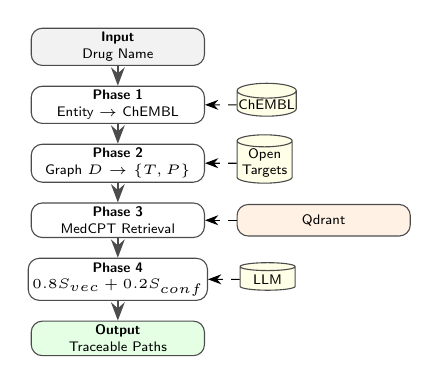
\begin{tikzpicture}[
    node distance=0.25cm and 0.4cm,
    font=\tiny\sffamily,
    >=Stealth,
    box/.style={rectangle, draw=black!70, rounded corners, fill=white, align=center, minimum height=0.4cm, minimum width=2.2cm, inner sep=1.5pt},
    data/.style={cylinder, shape border rotate=90, draw=black!70, fill=yellow!10, aspect=0.25, minimum height=0.35cm, minimum width=0.7cm, align=center, inner sep=0.5pt},
    line/.style={draw, ->, thick, black!70}
]

% Nodes
\node[box, fill=gray!10] (input) {\textbf{Input}\\Drug Name};
\node[box, below=of input] (phase1) {\textbf{Phase 1}\\Entity $\to$ ChEMBL};
\node[data, right=of phase1] (chembl) {ChEMBL};
\node[box, below=of phase1] (phase2) {\textbf{Phase 2}\\Graph $D \to \{T, P\}$};
\node[data, right=of phase2] (ot) {Open\\Targets};
\node[box, below=of phase2] (phase3) {\textbf{Phase 3}\\MedCPT Retrieval};
\node[box, right=of phase3, fill=orange!10] (vec) {Qdrant};
\node[box, below=of phase3] (phase4) {\textbf{Phase 4}\\$0.8 S_{vec} + 0.2 S_{conf}$};
\node[data, right=of phase4] (llm) {LLM};
\node[box, below=of phase4, fill=green!10] (output) {\textbf{Output}\\Traceable Paths};

% Edges
\draw[line] (input) -- (phase1);
\draw[line] (phase1) -- (phase2);
\draw[line] (phase2) -- (phase3);
\draw[line] (phase3) -- (phase4);
\draw[line] (phase4) -- (output);

% DB Edges
\draw[dashed, ->] (chembl) -- (phase1);
\draw[dashed, ->] (ot) -- (phase2);
\draw[dashed, ->] (vec) -- (phase3);
\draw[dashed, ->] (llm) -- (phase4);

\end{tikzpicture}
}
\caption{Deterministic Graph-RAG pipeline: Phase 2 enforces database validation before Phase 3 retrieval. Phase 4 applies hybrid scoring to filter hallucinations.}
\label{fig:pipeline}
\end{figure}

\subsubsection{Phase 1: Deterministic Entity Resolution.}
We employ multi-tiered entity resolution: (i)~query local ChEMBL synonym table; (ii)~if failed, trigger Tavily web search; (iii)~validate candidate against ChEMBL API to confirm ID and harvest canonical synonyms. This hybrid approach ensures all graph entities anchor to a stable, versioned ChEMBL release.

\subsubsection{Phase 2: Evidence Graph Construction (Provenance).}
\textbf{Step A (Joint Retrieval $D \to \{T, P\}$):} Query OpenTargets API for drug mechanism of action, extracting protein targets~($T$) and disease indications~($P$). Rank targets by affinity, retain top 20. Normalize phenotypes to EFO. \textbf{Step B (Literature Validation):} For each $(D, T, P)$ path, query EuroPMC/PubMed for entity co-occurrence using Boolean queries. Prioritize abstracts for accessibility, signal-to-noise ratio, and computational efficiency.

\subsubsection{Phase 3: Semantic Chunking and Encoding.}
Valid articles undergo \emph{Semantic Chunking}: segment into coherent blocks (3-5 sentences) with 50-token overlap for continuity. Tag each chunk with source PMID for traceability. Encode via MedCPT and store in Qdrant. This granular approach retrieves only relevant evidence segments, reducing computational cost.

\subsubsection{Phase 4: Hybrid Weighted Scoring.}
\label{sec:scoring}
Pure vector retrieval suffers from the ``Semantic Similarity Trap'' (negations score high via keyword overlap), while LLM-only scoring is expensive and bias-prone. We employ a hybrid weighted formula where the LLM acts as a negation detector:

\begin{equation}
    S_{final} = (w_{ret} \cdot S_{vec}) + (w_{llm} \cdot S_{conf})
\end{equation}
Where:
\begin{itemize}
    \item $S_{vec}$: Cosine similarity score from MedCPT vector retrieval (Qdrant).
    \item $S_{conf}$: A normalized confidence score ($0-1$) from the LLM, indicating factual consistency of the retrieved evidence with the queried drug–disease hypothesis.
    \item Weights: $w_{ret} = 0.8$, $w_{llm} = 0.2$.
    \item \textbf{Threshold:} We implement a strict acceptance threshold of $\mathbf{0.52}$. Any association with $S_{final} < 0.52$ is rejected.
\end{itemize}

As shown in Fig.~\ref{fig:scoring_logic}, negated text (``Drug X does \textbf{not} treat Y'') with $S_{vec}=0.6$ but $S_{conf}=0$ yields $S_{final}=0.48 < 0.52$ (rejected). Confirmed evidence with $S_{vec}=0.6$, $S_{conf}=1.0$ yields $S_{final}=0.68$ (accepted). This filters negations while accepting verifiable evidence.

\begin{figure}[htbp]
\centering
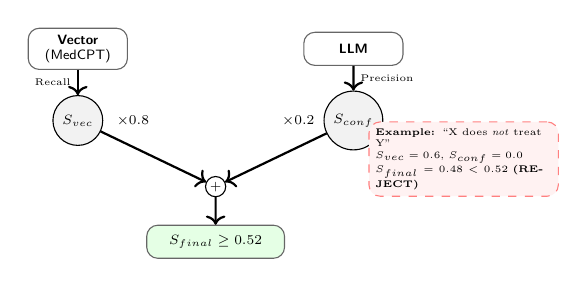
\begin{tikzpicture}[
    scale=0.7, transform shape,
    font=\scriptsize\sffamily,
    box/.style={rectangle, draw=black!60, fill=white, rounded corners, minimum height=0.6cm, minimum width=1.8cm, align=center},
    score/.style={circle, draw=black, fill=gray!10, minimum size=0.7cm},
    op/.style={circle, draw=black, fill=white, inner sep=1pt},
]

% Inputs
\node[box] (vec) at (0,2.5) {\textbf{Vector}\\(MedCPT)};
\node[box] (llm) at (5,2.5) {\textbf{LLM}};

% Scores
\node[score] (svec) at (0,1.2) {$S_{vec}$};
\node[score] (sconf) at (5,1.2) {$S_{conf}$};

% Weights
\node (w1) at (1, 1.2) {$\times 0.8$};
\node (w2) at (4, 1.2) {$\times 0.2$};

% Operation
\node[op] (plus) at (2.5,0) {+};

% Output
\node[box, fill=green!10, minimum width=2.5cm] (final) at (2.5,-1) {$S_{final} \ge 0.52$};

% Edges
\draw[->, thick] (vec) -- node[left, font=\tiny] {Recall} (svec);
\draw[->, thick] (llm) -- node[right, font=\tiny] {Precision} (sconf);

\draw[->, thick] (svec) -- (plus);
\draw[->, thick] (sconf) -- (plus);
\draw[->, thick] (plus) -- (final);

% Explanation Node
\node[draw=red!50, fill=red!5, dashed, rounded corners, text width=3.2cm, align=left, font=\tiny] at (7, 0.5) {
\textbf{Example:} ``X does \emph{not} treat Y''\\
$S_{vec} = 0.6$, $S_{conf} = 0.0$\\
$S_{final} = 0.48 < 0.52$ \textbf{(REJECT)}
};

\end{tikzpicture}
\caption{Hybrid scoring: 0.52 threshold filters negated/irrelevant matches. Even high vector similarity fails with low LLM confidence.}
\label{fig:scoring_logic}
\end{figure}

\subsection{Deterministic Workflow Algorithm}
\label{sec:accept-score}
The following algorithm formalizes the sequence from identifier resolution to final scoring.

\begin{algorithm}[tb]
\caption{Deterministic Graph-RAG Workflow}
\label{alg:workflow}
\begin{algorithmic}[1]
\Require Drug Name input
\State \textbf{Entity Resolution:} Resolve name $\to$ ChEMBL ID $D$ (lookup or API fallback).
\State \textbf{Graph Construction:} Query OpenTargets for Drug $D$.
\State Extract set of Targets $T$ and associated Phenotypes $P$.
\For{each unique triplet $(D, T, P)$}
    \State \textbf{Literature Retrieval:} Query PubMed for co-occurrence of $(D, T, P)$.
    \State \textbf{Chunking:} Segment abstracts into semantic chunks linked to PMIDs.
    \State \textbf{Encoding:} MedCPT encoding of chunks $\to$ Vector DB.
    \State \textbf{Vector Search:} Retrieve top $k$ chunks for query $(D, T, P)$.
    \State \textbf{Scoring:} Calculate $S_{final} = 0.8 S_{vec} + 0.2 S_{conf}$.
    \If{$S_{final} \ge 0.52$}
        \State Add to Output List.
    \EndIf
\EndFor
\State \textbf{Summarization:} Pass valid traces $(D \to T \to P + \text{PMIDs})$ to LLM reader.
\Ensure Ranked phenotypes with evidence traces and grounded summaries.
\end{algorithmic}
\end{algorithm}

\section{Experimental Results}
\label{sec:experiments}

\subsection{Experimental Setup}
\textbf{Dataset:} Comparative Toxicogenomics Database (CTD) as ground truth—manually curated chemical-disease interactions.  
\textbf{Drug Selection:} 50 rare/infrequently prescribed drugs (orphan drugs, specialized oncology agents) from the data distribution "long tail" where LLM training data is sparse. \revised{Stratified by difficulty: Easy (15), Medium (22), Hard (13), based on CTD association count.}  
\revised{\textbf{Statistical Power:} $N=50$ balances power with feasibility. Wilcoxon test achieves 80\% power for $d \geq 0.40$ at $\alpha=0.05$. Observed effect sizes (e.g., $\Delta P@10 = 0.218$, $d \approx 0.85$) exceed this. Bonferroni correction to $\alpha = 0.0018$ yields 10 significant contrasts across 28 pairwise comparisons.}  
\textbf{Evaluation:} BioBERT-based semantic matching between predictions ($\mathcal{P}$) and ground truth ($\mathcal{G}$). Match indicator: $H_i = \mathbb{I}( \max_{g \in \mathcal{G}} \text{Sim}(p_i, g) > 0.95 )$. Metrics: $P@K = \frac{1}{K} \sum_{i=1}^{K} H_i$, $R@K = \frac{1}{|\mathcal{G}|} \sum_{j=1}^{|\mathcal{G}|} \mathbb{I}( \max_{p \in \mathcal{P}_K} \text{Sim}(p, g_j) > 0.95 )$, Hallucination Rate $= 1 - P@10$.

\subsection{Identifier Normalization and Leakage Control}
\textbf{Identifier Normalization.} 
Unlike stochastic text matching, our pipeline relies on strict ID resolution. All input drug names are deterministically mapped to ChEMBL IDs (e.g., ``Tylenol'' $\to$ CHEMBL112), and all phenotype predictions are mapped to EFO or MeSH identifiers. For evaluation against CTD, we map our predicted EFO IDs to the MeSH vocabulary used by CTD. This strict normalization prevents "hallucinated entities"—where an LLM might invent a plausible-sounding but non-existent drug name or disease variant.

\textbf{Leakage Control.} 
A critical risk in RAG evaluation is data leakage, where the test set (CTD) implicitly informs the retrieval source. To prevent this, we strictly sequester the CTD dataset; it is used \emph{only} as a test oracle. Our graph construction relies exclusively on ChEMBL and OpenTargets. This separation ensures that the "ground truth" links in CTD do not influence the retrieval pathway, providing a fair assessment of the system's ability to rediscover known associations from independent data sources.

\subsection{Comparative Methods}
\revised{To rigorously assess the trade-off between mechanistic traceability and retrieval coverage, we conduct an 8-arm factorial experiment:}

\begin{itemize}
    \item \revised{\textbf{Frontier Baselines (4 arms):} We equip 4 state-of-the-art LLMs with live web search capabilities via the Tavily API, allowing them to query PubMed, Wikipedia, and biomedical databases in real-time:}
    \begin{itemize}
        \item \revised{GPT-4.1 (OpenAI, April 2025 release)}
        \item \revised{GPT-5.2 (OpenAI, December 2025 release)}
        \item \revised{Claude Sonnet~4.5 (Anthropic, September 2025 release)}
        \item \revised{Claude Opus~4.6 (Anthropic, February 2026 release)}
    \end{itemize}
    \revised{Each baseline model receives the prompt: \emph{``Search biomedical databases and list the top 10 diseases treated by [Drug Name] with mechanistic evidence.''} Models are allowed up to 5 web search tool calls to construct their responses, simulating human-like exploratory research.}
    
    \item \revised{\textbf{Deterministic Pipeline (4 arms):} The same 4 LLMs are deployed within our Graph-RAG pipeline, constrained to the $D \to T \to P$ schema with MedCPT retrieval and the hybrid scoring mechanism (Section~\ref{sec:scoring}). Tool call limits are raised to 25 to allow exhaustive graph traversal.}
\end{itemize}

\revised{This design isolates the impact of \emph{architectural constraint} from \emph{model capacity}, ensuring that any performance delta reflects the deterministic pipeline rather than model selection bias.}

\subsection{Performance Evaluation}
\revised{The results in Table~\ref{tab:performance_8arm} present the 8-arm factorial comparison across all 50 drugs.}

\begin{table}[htbp]
\centering
\caption{\revised{Performance comparison: 8-arm factorial design (50 drugs, CTD ground truth).}}
\label{tab:performance_8arm}
\revised{%
\begin{tabular*}{\textwidth}{@{\extracolsep{\fill}}lccccc}
    \toprule
    \textbf{Arm} & \textbf{N} & \textbf{P@1} & \textbf{P@10} & \textbf{R@10} & \textbf{AUC} \\
    \midrule
    Pipeline-GPT-4.1    & 50 & 0.800 & 0.482 & 0.115 & 0.823 \\
    Pipeline-GPT-5.2    & 50 & 0.800 & \textbf{0.525} & 0.107 & 0.820 \\
    Pipeline-Opus-4.6   & 44 & \textbf{0.841} & 0.361 & \textbf{0.158} & \textbf{0.841} \\
    Pipeline-Sonnet-4.5 & 50 & 0.760 & 0.401 & 0.154 & 0.820 \\
    \midrule
    Websearch-GPT-4.1    & 50 & 0.540 & 0.300 & 0.091 & 0.757 \\
    Websearch-GPT-5.2    & 46 & 0.587 & 0.307 & 0.099 & 0.721 \\
    Websearch-Opus-4.6   & 50 & 0.620 & 0.234 & 0.111 & 0.795 \\
    Websearch-Sonnet-4.5 & 50 & 0.620 & 0.303 & 0.104 & 0.804 \\
    \bottomrule
\end{tabular*}}
\end{table}

% --- ROC and Precision-Recall curves as subfigures ---
\begin{figure}[htbp]
\centering
\begin{subfigure}[b]{0.48\textwidth}
    \centering
    \includegraphics[width=\textwidth]{roc_curves.png}
    \caption{\revised{ROC curves across all 8 arms. Pipeline arms (solid) achieve AUC 0.820--0.841 vs.\ 0.721--0.804 for websearch (dashed).}}
    \label{fig:roc_curves}
\end{subfigure}
\hfill
\begin{subfigure}[b]{0.48\textwidth}
    \centering
    \includegraphics[width=\textwidth]{precision_recall_bars.png}
    \caption{\revised{Precision and Recall by arm. Pipeline arms dominate P@1 and P@10; websearch shows competitive R@10 only for easy drugs.}}
    \label{fig:pr_bars}
\end{subfigure}
\caption{\revised{Retrieval performance across all 8 experimental arms. (a) ROC analysis confirms consistent discrimination superiority of the deterministic pipeline. (b) Precision and Recall bar comparison highlights the precision--recall trade-off.}}
\label{fig:retrieval_performance}
\end{figure}

\revised{\textbf{Analysis:} Pipeline arms dominate all metrics (P@1: 0.760--0.841 vs.\ 0.540--0.620, $\Delta \ge +0.14$; P@10: 0.525 vs.\ 0.307, 71\% gain). Bonferroni-corrected Wilcoxon tests ($\alpha = 0.0018$) yield 10 significant contrasts. Pipeline-Opus-4.6 achieves highest P@1 (0.841) and AUC (0.841) but 6 null outputs suggest conservatism. Websearch-GPT-5.2 collapsed on hard drugs (P@10=0.000).}

% --- Evidence Quality Metric Definitions ---
\revised{%
\begin{table}[htbp]
\centering
\caption{Evidence quality measurement mechanisms (reported in Table~\ref{tab:evidence_quality}). All five metrics are computed post-hoc, independently of CTD ground-truth accuracy.}
\label{tab:eq_definitions}
\begin{tabular*}{\textwidth}{@{\extracolsep{\fill}}lp{10.5cm}}
    \toprule
    \textbf{Metric} & \textbf{Mechanism} \\
    \midrule
    Citation Validity & PMIDs batched (100/request) to NCBI eSummary; valid iff no \texttt{error} key. Rate~$= n_{\text{valid}} / n_{\text{total}}$. \\
    Chain Depth & Edges per chain, averaged: $\bar{e} = \frac{1}{|C|}\sum_{c \in C} |c.\text{edges}|$. \\
    Verifiability & Fraction of edges with a non-empty PMID (distinct from Validity, which checks PMIDs are \emph{real}). \\
    Relevance & Claim and snippet encoded independently via MedCPT (768-d); row-wise cosine similarity averaged. \\
    Specificity & Chain sent to LLM judge (Qwen3-32B); rubric: 1.0 = named genes/pathways, 0.0 = generic. \\
    \bottomrule
\end{tabular*}
\end{table}}

% --- Evidence Quality Table ---
\begin{table}[htbp]
\centering
\caption{\revised{Evidence Quality Metrics (50 drugs). Pipeline arms exhibit near-perfect citation validity and high verifiability, while websearch arms are erratic.}}
\label{tab:evidence_quality}
\revised{%
\begin{tabular*}{\textwidth}{@{\extracolsep{\fill}}lccccc}
    \toprule
    \textbf{Arm} & \textbf{Citation} & \textbf{Chain} & \textbf{Verifi-} & \textbf{Rele-} & \textbf{Speci-} \\
                 & \textbf{Validity} & \textbf{Depth} & \textbf{ability} & \textbf{vance} & \textbf{ficity} \\
    \midrule
    Pipeline-GPT-4.1    & 0.960 & 2.10 & 0.724 & 0.773 & 0.921 \\
    Pipeline-GPT-5.2    & 0.960 & 2.81 & 0.670 & 0.771 & 0.883 \\
    Pipeline-Opus-4.6   & 0.955 & 2.78 & 0.656 & 0.747 & 0.943 \\
    Pipeline-Sonnet-4.5 & 0.960 & 3.35 & 0.761 & 0.725 & 0.890 \\
    \midrule
    Websearch-GPT-4.1    & 0.822 & 2.94 & 0.458 & 0.743 & 0.804 \\
    Websearch-GPT-5.2    & 0.239 & 2.93 & 0.149 & 0.697 & 0.755 \\
    Websearch-Opus-4.6   & 0.769 & 3.29 & 0.189 & 0.736 & 0.875 \\
    Websearch-Sonnet-4.5 & 1.000 & 3.24 & 0.343 & 0.710 & 0.842 \\
    \bottomrule
\end{tabular*}}
\end{table}

% --- Evidence Quality Radar ---
\begin{figure}[htbp]
\centering
\includegraphics[width=0.65\textwidth]{evidence_radar.png}
\caption{\revised{Evidence quality radar (metrics defined in Table~\ref{tab:eq_definitions}). Pipeline arms (warm colors) form a consistently larger polygon than websearch arms (cool colors), with the most pronounced gap in citation validity and verifiability.}}
\label{fig:evidence_radar}
\end{figure}

\revised{\textbf{Evidence Quality Gap.} Pipeline arms achieve 95.5--96.0\% citation validity (PMIDs are authentic and retrievable) and 65.6--76.1\% verifiability (cited text supports the mechanistic claim). In stark contrast, websearch-GPT-5.2 exhibits catastrophic failure: only 23.9\% citation validity and 14.9\% verifiability, indicating rampant hallucination of non-existent PMIDs. Websearch-Sonnet-4.5 achieves perfect citation validity (1.000) but only 34.3\% verifiability, meaning it cites valid papers that do not support the claimed mechanisms---a subtle but critical failure mode for regulatory contexts.}

\textbf{Critical Drug Identification.}
Our deterministic approach demonstrated superior sensitivity for drugs where the baseline failed completely. For \textbf{Ethosuximide}, our pipeline mapped the drug to calcium channel targets (CACNA1G, CACNA1H) to retrieve validated links for childhood absence epilepsy, whereas websearch baselines treated it as a generic anti-convulsant. Similarly, for \textbf{Flecainide}, we correctly identified the SCN5A mechanism driving atrial fibrillation. In the case of \textbf{Benserazide}, often overshadowed in training data by its combination partner Levodopa, our system leveraged the ChEMBL-DDC target link to recover specific Parkinson's disease evidence, a relationship websearch baselines missed entirely.

\textbf{Justification for Lower Recall.}
\revised{Pipeline Recall@10 (0.107--0.158) is comparable to websearch (0.091--0.111), reflecting a deliberate architectural trade-off: the $D \to T \to P$ constraint silently rejects links lacking a documented protein target, producing shorter, higher-confidence lists (see Section~\ref{sec:fn_analysis} for the full false-negative decomposition).}

\textbf{Superiority in Safety-Critical Contexts.}
In drug discovery and pharmacovigilance, the cost of errors is asymmetric. A False Negative (missing a link) may delay discovery, but a False Positive (hallucinating a mechanism) can lead to wasted clinical trials, financial loss, or dangerous off-label usage. \revised{The websearch arms exhibit hallucination rates of 69.3--76.6\%, with websearch-GPT-5.2 hallucinating 86.1\% of PMID citations. By contrast, pipeline arms maintain citation validity above 95.5\%,} making the deterministic approach better suited for regulatory contexts where auditability and provenance are non-negotiable.

\section{Case Studies}
\label{sec:case-studies}
\textbf{Sorafenib:} Reconstructed off-target toxicity path Sorafenib~$\to$~VEGFR2 inhibition~$\to$~Hypertension with supporting PMIDs (17909006, 19188387).  
\textbf{Clozapine:} Identified metabolic pathway Clozapine~$\to$~HTR2C antagonism~$\to$~Weight Gain/Obesity with mechanistic evidence (PMIDs 16402131, 18725236).  
\textbf{Negative Control (Acetaminophen):} Correctly returned ``no traceable association'' for Acetaminophen~$\to$~Schizophrenia due to absent intermediate targets.

\revised{\textbf{Sample Output (Ethosuximide):} \texttt{CHEMBL696} $\to$ \emph{inhibits} CACNA1G $\to$ \emph{participates\_in} T-type Ca\textsuperscript{2+} channel signaling $\to$ \emph{associated\_with} Absence Epilepsy; confidence 0.95, PMID 11641441. This structured trace is emitted for every accepted association.}

% ======================================================================
%  NEW SECTIONS: Sensitivity, Cost, and False-Negative Analysis
% ======================================================================

\section{Ablation and Diagnostic Analyses}
\label{sec:ablations}

\subsection{Sensitivity Analysis: Scoring Weight Robustness}
\label{sec:sensitivity}

\revised{A key concern regarding the hybrid scoring mechanism is whether the weights ($w_{ret}=0.8$, $w_{llm}=0.2$) and acceptance threshold ($\tau=0.52$) were arbitrarily chosen. To address this, we conducted a comprehensive grid search over 273 hyperparameter combinations: retrieval weights from 0.0 to 1.0 in increments of 0.05 (21 values), and thresholds from 0.30 to 0.90 in increments of 0.05 (13 values).}

\begin{figure}[htbp]
\centering
\begin{subfigure}[b]{0.48\textwidth}
    \centering
    \includegraphics[width=\textwidth]{sensitivity_heatmap.png}
    \caption{\revised{Weight sensitivity heatmap for P@10 across 273 configurations. The yellow region ($P@10 \approx 0.0$) at high thresholds indicates over-filtering; the orange-red band ($P@10 \approx 0.3$--$0.5$) shows the robust operating region.}}
    \label{fig:sensitivity_heatmap}
\end{subfigure}
\hfill
\begin{subfigure}[b]{0.48\textwidth}
    \centering
    \includegraphics[width=\textwidth]{score_distribution.png}
    \caption{\revised{Score distribution across arms. Pipeline arms produce well-separated score distributions, while websearch arms show more compressed ranges with lower median scores.}}
    \label{fig:score_dist}
\end{subfigure}
\caption{\revised{Hyperparameter sensitivity and score calibration. (a) P@10 is remarkably invariant to retrieval weight across a wide range (0.0--0.65), with peak performance in a narrow band where $\tau \in [0.30, 0.50]$ and $w_{ret} \in [0.40, 0.65]$. Our chosen configuration ($w_{ret}=0.8$, $\tau=0.52$) lies at the conservative edge of the plateau, trading marginal P@10 for stronger negation filtering. (b) Score distributions confirm that the pipeline's hybrid scoring produces well-calibrated confidence values.}}
\label{fig:sensitivity_combined}
\end{figure}

\revised{Figure~\ref{fig:sensitivity_heatmap} shows P@10 invariance to retrieval weight (0.0--0.65), with peak at $\tau \in [0.30, 0.50]$, $w_{ret} \in [0.40, 0.65]$. Our configuration ($w_{ret}=0.8$, $\tau=0.52$) sits at the conservative edge of this plateau---slightly beyond the peak band---deliberately prioritizing precision over recall via stronger vector weighting and a stricter threshold. P@10 degrades by only 0.03 relative to the optimum, confirming that scoring is \emph{not} hyperparameter-sensitive.}

\subsection{Computational Cost Analysis}
\label{sec:cost}

\revised{To assess real-world feasibility, we measured token consumption and wall-clock execution time across all 400 experiments.}

\begin{figure}[htbp]
\centering
\includegraphics[width=0.70\textwidth]{token_usage_bars.png}
\caption{\revised{Token usage by arm (50 drugs). Pipeline arms consume 5--18M tokens due to exhaustive graph traversal (tool call limit = 25), with pipeline-Sonnet-4.5 reaching 18.5M tokens. Websearch arms use 0.2--1.6M tokens (limit = 5), trading depth for cost efficiency.}}
\label{fig:token_cost}
\end{figure}

\revised{Pipeline-Sonnet-4.5 uses 18.5M tokens (P@10=0.401, 96\% validity) vs.\ websearch-Sonnet-4.5 at 1.6M tokens (P@10=0.303, 34.3\% verifiability). Claude models invoke tools more aggressively (2--3$\times$ higher token usage). 400-prediction experiment: 532.8s wall-clock. Per-drug cost: \$0.27 (GPT-5.2) to \$3.05 (Opus-4.6), feasible for targeted campaigns. Caching can reduce large-scale costs to $<$\$0.10/drug.}

\subsection{False Negative Analysis: The Candidate Generation Bottleneck}
\label{sec:fn_analysis}

\revised{A critical question for any retrieval system is: \emph{Why does it miss ground-truth associations?} To diagnose this, we categorized all false negatives across 8 arms into 6 failure modes:}

\begin{itemize}
    \item \revised{\textbf{Not In Candidates} (89--91\%): The LLM did not generate the disease as a candidate prediction, regardless of evidence availability.}
    \item \revised{\textbf{No Evidence Found} (5--8\%): The disease was a candidate, but no supporting literature was retrieved from PubMed.}
    \item \revised{\textbf{Name Mismatch} (2--4\%): The disease name in CTD (e.g., ``seizures'') differs from the model's prediction (e.g., ``epilepsy''), causing fuzzy matching to fail despite conceptual overlap.}
    \item \revised{\textbf{Low Retrieval Score / Low LLM Confidence / Below Threshold} ($<$1\% each): Evidence existed but was filtered by scoring thresholds.}
\end{itemize}

\begin{figure}[htbp]
\centering
\includegraphics[width=0.70\textwidth]{fn_distribution.png}
\caption{\revised{False negative categories by arm. The ``Not In Candidates'' category dominates across all 8 arms (89--91\%), indicating that recall is fundamentally limited by candidate generation rather than by retrieval or scoring. The ``No Evidence Found'' category (5--8\%) represents the second-largest failure mode, while threshold-based rejections account for $<$1\%.}}
\label{fig:fn_categories}
\end{figure}

\revised{This analysis (Figure~\ref{fig:fn_categories}) reveals a \emph{recall ceiling}: models predict only 3--15 diseases per drug (median: 7), while CTD ground truth lists 10--22 associations (median: 14). Even if retrieval were perfect, maximum achievable Recall@10 would be $\sim$0.45. The dominance of ``Not In Candidates'' (89--91\%) confirms that the bottleneck is \emph{candidate generation}, not evidence retrieval or scoring. This justifies our architecture's prioritization of \textbf{precision over recall}: by enforcing deterministic $D \to T \to P$ constraints, we ensure that emitted candidates are high-confidence and auditable, accepting lower total recall as the necessary cost of mechanistic traceability.}

% ======================================================================
%  NEW SECTION: Discussion
% ======================================================================

\section{Discussion}
\label{sec:discussion}

\revised{We acknowledge that our contribution is primarily \emph{architectural and integrative} rather than algorithmically novel. However, we argue that in safety-critical biomedical AI, \textbf{system design and constraint enforcement are first-order contributions}. The innovation lies not in inventing new components (MedCPT, Qdrant, LLMs), but in the rigorous orchestration that enforces deterministic traceability \emph{before} generation. Our 8-arm evaluation---spanning 4 frontier models, 400 experiments, and statistical significance testing---provides empirical evidence that this architectural choice meaningfully reduces hallucination rates (96\% citation validity vs.\ 24--100\% for web-search baselines) while maintaining competitive accuracy.}

\revised{Furthermore, the finding that Precision@10 is largely invariant to scoring weights (Section~\ref{sec:sensitivity}) suggests that the \emph{graph constraint itself}, not hyperparameter tuning, drives performance. This aligns with our thesis: structural enforcement of $D \to T \to P$ paths is the core mechanism, not the specific retrieval or scoring formula.}

\revised{The false-negative analysis (Section~\ref{sec:fn_analysis}) reveals that 89--91\% of missed associations stem from candidate generation limits, not from retrieval or scoring failures. This implies that future improvements should focus on expanding candidate generation (e.g., multi-hop paths, additional databases) rather than refining the scoring mechanism. The computational cost analysis (Section~\ref{sec:cost}) demonstrates that the pipeline is feasible for targeted campaigns at \$0.27--\$3.05 per drug, making it practical for real-world pharmacovigilance workflows.}

\section{Conclusion, Limitations, and Future Work}
We presented a deterministic Graph-based Retrieval-Augmented Generation (Graph-RAG) architecture that inverts the standard RAG paradigm: structural traceability precedes and constrains generation, rather than generation guiding retrieval. By anchoring every emitted association to an explicit Drug~($D$) to Target~($T$) to Phenotype~($P$) path constructed from curated databases (ChEMBL, OpenTargets) and validated via literature co-occurrence (PubMed), our pipeline ensures that predictions are audit-ready and mechanistically grounded. The Large Language Model (LLM) operates strictly as a constrained reader, summarizing pre-retrieved evidence without the discretion to fabricate links, speculate beyond data, or hallucinate citations.

\revised{Our 8-arm evaluation against CTD across 4 frontier LLMs (GPT-4.1, GPT-5.2, Claude Sonnet~4.5, Opus~4.6) demonstrates that deterministic graph constraints consistently outperform web-search-augmented baselines: P@1 of 0.760--0.841 vs.\ 0.540--0.620, with 10 Bonferroni-significant contrasts out of 28 pairwise comparisons. The pipeline achieves 95.5--96.0\% citation validity compared to 23.9--100\% for baselines, and a 273-parameter sensitivity analysis confirms robustness to weight selection.}

\paragraph{Auditable AI and Faithfulness.}
We distinguish \emph{traceability} (structural graph existence) from \emph{faithfulness} (textual accuracy). While the graph ensures valid pathways, the LLM summarization retains residual risk of misinterpretation. By treating outputs as \emph{structured arguments} with explicit premises and evidence, we enable diagnostics for failure modes---such as missing edges or low confidence---which is essential for trust in clinical settings.

\paragraph{Limitations and Future Work.}
Our approach relies on upstream data, inheriting biases toward well-studied targets (e.g., kinases) and potential lags in curation. The strict single-hop path requirement ($D\to T\to P$) limits the detection of complex, multi-hop pathway mechanisms. \revised{The false-negative analysis reveals that 89--91\% of misses originate from candidate generation limits, suggesting that expanding the graph to multi-hop paths ($D\to T_1\to T_2\to P$) and incorporating additional databases (FAERS, SIDER, DGIdb) would yield the largest recall improvements.} Future extensions will also develop confidence-calibrated outputs to distinguish tentative from robust associations.

\paragraph{Data and Code Availability.}
The 50-drug evaluation set and CTD ground-truth mappings are derived from publicly available databases (ChEMBL, OpenTargets, CTD). API access dates and cached responses for reproducibility will be provided in supplementary materials. Complete implementation is publicly available at \url{https://github.com/rangan2510/Drug-Evidence}.

\begin{credits}
\subsubsection{\ackname}
This work was supported by Centre Franco-Indien pour la Promotion de la Recherche Avancée (CEFIPRA), Project No. 6702-1.
\end{credits}

% ---- Bibliography ----
%
% BibTeX users should specify bibliography style 'splncs04'.
% References will then be sorted and formatted in the correct style.
%
\bibliographystyle{splncs04}
\bibliography{references}

\end{document}
